

\documentclass{article}
\usepackage[utf8]{inputenc}
\usepackage[utf8]{inputenc}
\usepackage[T1]{fontenc}
\usepackage[english]{babel}
\usepackage{fullpage}
\usepackage{color}
\usepackage[table]{xcolor}
\usepackage{listings}
 
\definecolor{darkWhite}{rgb}{0.94,0.94,0.94}
 
\lstset{
  aboveskip=3mm,
  belowskip=-2mm,
  backgroundcolor=\color{darkWhite},
  basicstyle=\footnotesize,
  breakatwhitespace=false,
  breaklines=true,
  captionpos=b,
  commentstyle=\color{red},
  deletekeywords={...},
  escapeinside={\%*}{*)},
  extendedchars=true,
  framexleftmargin=16pt,
  framextopmargin=3pt,
  framexbottommargin=6pt,
  frame=tb,
  keepspaces=true,
  keywordstyle=\color{blue},
  language=C,
  literate=
  {²}{{\textsuperscript{2}}}1
  {⁴}{{\textsuperscript{4}}}1
  {⁶}{{\textsuperscript{6}}}1
  {⁸}{{\textsuperscript{8}}}1
  {€}{{\euro{}}}1
  {é}{{\'e}}1
  {è}{{\`{e}}}1
  {ê}{{\^{e}}}1
  {ë}{{\¨{e}}}1
  {É}{{\'{E}}}1
  {Ê}{{\^{E}}}1
  {û}{{\^{u}}}1
  {ù}{{\`{u}}}1
  {â}{{\^{a}}}1
  {à}{{\`{a}}}1
  {á}{{\'{a}}}1
  {ã}{{\~{a}}}1
  {Á}{{\'{A}}}1
  {Â}{{\^{A}}}1
  {Ã}{{\~{A}}}1
  {ç}{{\c{c}}}1
  {Ç}{{\c{C}}}1
  {õ}{{\~{o}}}1
  {ó}{{\'{o}}}1
  {ô}{{\^{o}}}1
  {Õ}{{\~{O}}}1
  {Ó}{{\'{O}}}1
  {Ô}{{\^{O}}}1
  {î}{{\^{i}}}1
  {Î}{{\^{I}}}1
  {í}{{\'{i}}}1
  {Í}{{\~{Í}}}1,
  morekeywords={*,...},
  numbers=left,
  numbersep=10pt,
  numberstyle=\tiny\color{black},
  rulecolor=\color{black},
  showspaces=false,
  showstringspaces=false,
  showtabs=false,
  stepnumber=1,
  stringstyle=\color{gray},
  tabsize=4,
  title=\lstname,
}
\usepackage{graphicx}
\graphicspath{ {./images/} }
\title{HAI804I – Analyse et Traitement d'Images}
\author{Fabien Caballero }

\begin{document}  

\maketitle
    \tableofcontents

\newpage

\section{Seuillage}
Pour réaliser cela, je parcours tout mes voxels un par un, pour chacun d'entre eux je regarde si sa valeur est supérieure au seuil si ce n'est pas le cas on passe au suivant. Si c'est le cas on récupère tout les voxels voisins (les 6) et pour chacun des voisins on regarde si leur valeur est inférieure au seuil si c'est le cas on ajoute la face qu'ils ont en commun dans le fichier stl.
Puis on écrit le fichier stl et on l'ouvre avec meshlab par exemple, pour le visionner. 

\begin{figure}[h]
\centerline{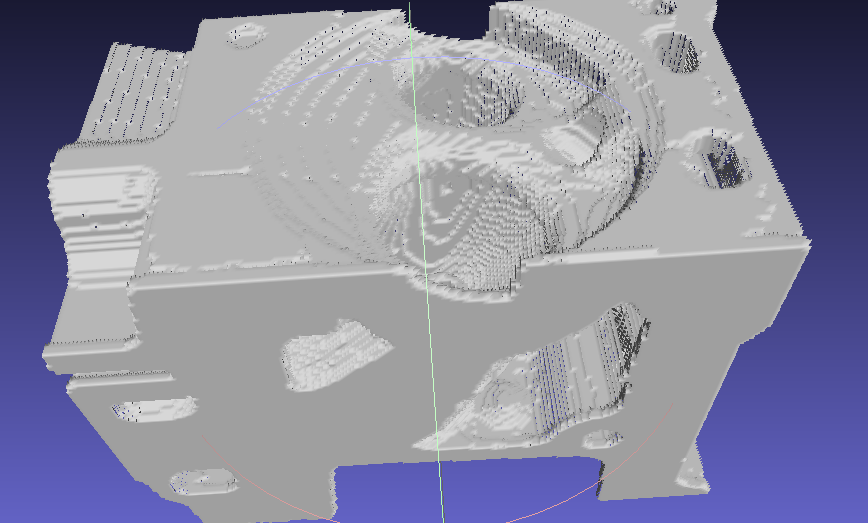
\includegraphics[scale=0.38]{./100.png}}
\caption{Engine seuil 100}

\centerline{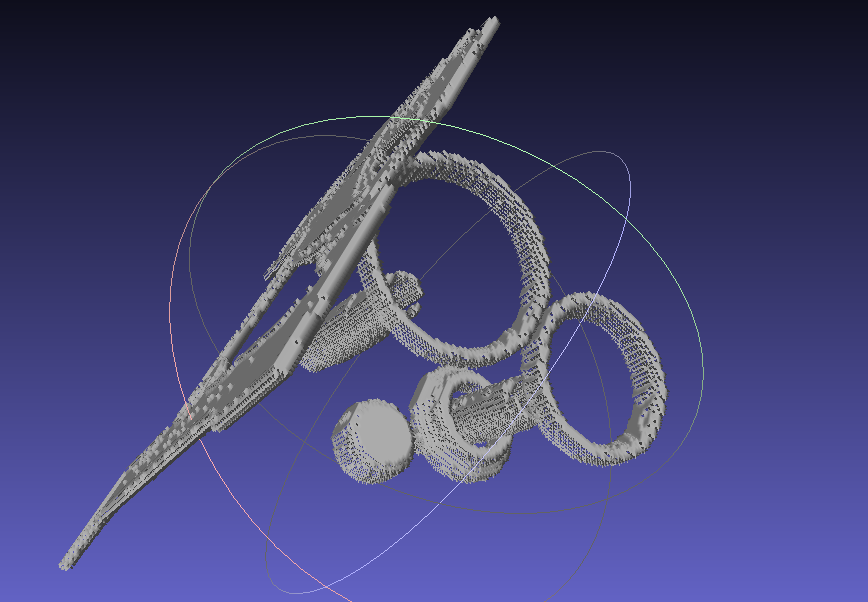
\includegraphics[scale=0.38]{./200.png}}
\caption{Engine seuil 200}
\end{figure}

\newpage
\section{Ce qu'il me reste à faire}
Je n'ai pas eu le temps de faire pour les autres fichiers, je ne peux donc pas vérifier si c'est bon lorsque les voxels ne sont pas cubiques.
Cependant je l'ai normalement géré en multipliant par la taille de mes voxels lors de la créations des sommets de mes voxels. Les tailles des voxels sont définies dans le code avec des variables je n'ai pas eu le temps de les mettres en paramètre de la ligne de commande.
\newpage

\section{Annexe (code)}
\begin{lstlisting}
    #include <stdio.h>
#include <iostream>
#include "image_ppm.h"
#include <vector>
#include <fstream>
using namespace std;

unsigned short getValue(unsigned short *img, int x, int y, int z, int dimX, int dimY, int dimZ)
{
    return (int)img[z * dimY * dimX + y * dimX + x];
}

unsigned short minElmt(unsigned short *img, size_t taille)
{
    unsigned short min = 0;
    for (size_t i = 0; i < taille; i++)
    {
        if (img[i] < min)
            min = img[i];
    }
    return min;
}

unsigned short maxElmt(unsigned short *img, size_t taille)
{
    unsigned short max = 0;
    for (size_t i = 0; i < taille; i++)
    {
        if (img[i] > max)
            max = img[i];
    }
    return max;
}

unsigned short inverse(unsigned short val)
{
    float o1 = floor(((double)val / 256.0));
    float o2 = val - o1 * 256;

    return o2 * 256 + o1;
}

vector<vector<int>> voisinage6(int i, int j, int k)
{
    vector<vector<int>> voisinage = {{i - 1, j, k}, {i + 1, j, k}, {i, j - 1, k}, {i, j + 1, k}, {i, j, k - 1}, {i, j, k + 1}};

    return voisinage;
}

int main(int argc, char const *argv[])
{
    FILE *f = fopen((char *)argv[1], "rb");
    unsigned short *contenu;

    int dimX = atoi(argv[2]);
    int dimY = atoi(argv[3]);
    int dimZ = atoi(argv[4]);

    int seuil = atoi(argv[5]);
    allocation_tableau(contenu, unsigned short, dimX *dimY *dimZ);

    size_t taille = fread(contenu, sizeof(unsigned short), dimX * dimY * dimZ, f);
    for (size_t i = 0; i < taille; i++)
    {
        contenu[i] = inverse(contenu[i]);
    }

    int voxelSizeX = 1;
    int voxelSizeY = 1;
    int voxelSizeZ = 1;
    

    ofstream file;
    file.open("modelbis.stl");
    file << "solid modelbis.stl" << endl;

    for (size_t i = 1; i < dimX - 1; i++)
    {
        for (size_t j = 1; j < dimY - 1; j++)
        {
            for (size_t k = 1; k < dimZ - 1; k++)
            {
                if (getValue(contenu, i, j, k, dimX, dimY, dimZ) < seuil)
                {
                    continue;
                }
                vector<vector<int>> vect = voisinage6(i, j, k);
                size_t size = vect.size();
                for (size_t v = 0; v < 6; v++)
                {
                    if (getValue(contenu, vect[v][0], vect[v][1], vect[v][2], dimX, dimY, dimZ) < seuil)
                    {
                        vector<float> center = {(float)vect[v][0], (float)vect[v][1], (float)vect[v][2]};
                        vector<float> zero = {(center[0] - 0.5f) * voxelSizeX, (center[1] - 0.5f) * voxelSizeY, (center[2] + 0.5f) * voxelSizeZ};
                        vector<float> un = {(center[0] + 0.5f) * voxelSizeX, (center[1] - 0.5f) * voxelSizeY, (center[2] - 0.5f) * voxelSizeZ};
                        vector<float> deux = {(center[0] + 0.5f) * voxelSizeX, (center[1] - 0.5f) * voxelSizeY, (center[2] - 0.5f) * voxelSizeZ};
                        vector<float> trois = {(center[0] - 0.5f) * voxelSizeX, (center[1] - 0.5f) * voxelSizeY, (center[2] - 0.5f) * voxelSizeZ};
                        vector<float> quatre = {(center[0] - 0.5f) * voxelSizeX, (center[1] + 0.5f) * voxelSizeY, (center[2] + 0.5f) * voxelSizeZ};
                        vector<float> cinq = {(center[0] + 0.5f) * voxelSizeX, (center[1] + 0.5f) * voxelSizeY, (center[2] + 0.5f) * voxelSizeZ};
                        vector<float> six = {(center[0] + 0.5f) * voxelSizeX, (center[1] + 0.5f) * voxelSizeY, (center[2] - 0.5f) * voxelSizeZ};
                        vector<float> sept = {(center[0] - 0.5f) * voxelSizeX, (center[1] + 0.5f) * voxelSizeY, (center[2] - 0.5f) * voxelSizeZ};
                        switch (v)
                        {
                        case 1:

                            file << "facet normal 0 0 0" << endl;
                            file << "\touter loop" << endl;
                            file << "\t\tvertex " << zero[0] << " " << zero[1] << " " << zero[2] << endl;
                            file << "\t\tvertex " << trois[0] << " " << trois[1] << " " << trois[2] << endl;
                            file << "\t\tvertex " << quatre[0] << " " << quatre[1] << " " << quatre[2] << endl;

                            file << "\tendloop" << endl;
                            file << "endfacet" << endl;

                            file << "facet normal 0 0 0" << endl;
                            file << "\touter loop" << endl;
                            file << "\t\tvertex " << trois[0] << " " << trois[1] << " " << trois[2] << endl;
                            file << "\t\tvertex " << sept[0] << " " << sept[1] << " " << sept[2] << endl;
                            file << "\t\tvertex " << quatre[0] << " " << quatre[1] << " " << quatre[2] << endl;

                            file << "\tendloop" << endl;
                            file << "endfacet" << endl;
                            break;
                        case 2:

                            file << "facet normal 0 0 0" << endl;
                            file << "\touter loop" << endl;
                            file << "\t\tvertex " << un[0] << " " << un[1] << " " << un[2] << endl;
                            file << "\t\tvertex " << deux[0] << " " << deux[1] << " " << deux[2] << endl;
                            file << "\t\tvertex " << cinq[0] << " " << cinq[1] << " " << cinq[2] << endl;

                            file << "\tendloop" << endl;
                            file << "endfacet" << endl;

                            file << "facet normal 0 0 0" << endl;
                            file << "\touter loop" << endl;
                            file << "\t\tvertex " << deux[0] << " " << deux[1] << " " << deux[2] << endl;
                            file << "\t\tvertex " << six[0] << " " << six[1] << " " << six[2] << endl;
                            file << "\t\tvertex " << cinq[0] << " " << cinq[1] << " " << cinq[2] << endl;

                            file << "\tendloop" << endl;
                            file << "endfacet" << endl;
                            break;
                        case 3:

                            file << "facet normal 0 0 0" << endl;
                            file << "\touter loop" << endl;
                            file << "\t\tvertex " << zero[0] << " " << zero[1] << " " << zero[2] << endl;
                            file << "\t\tvertex " << un[0] << " " << un[1] << " " << un[2] << endl;
                            file << "\t\tvertex " << trois[0] << " " << trois[1] << " " << trois[2] << endl;

                            file << "\tendloop" << endl;
                            file << "endfacet" << endl;

                            file << "facet normal 0 0 0" << endl;
                            file << "\touter loop" << endl;
                            file << "\t\tvertex " << un[0] << " " << un[1] << " " << un[2] << endl;
                            file << "\t\tvertex " << deux[0] << " " << deux[1] << " " << deux[2] << endl;
                            file << "\t\tvertex " << trois[0] << " " << trois[1] << " " << trois[2] << endl;

                            file << "\tendloop" << endl;
                            file << "endfacet" << endl;
                            break;
                        case 4:

                            file << "facet normal 0 0 0" << endl;
                            file << "\touter loop" << endl;
                            file << "\t\tvertex " << quatre[0] << " " << quatre[1] << " " << quatre[2] << endl;
                            file << "\t\tvertex " << cinq[0] << " " << cinq[1] << " " << cinq[2] << endl;
                            file << "\t\tvertex " << sept[0] << " " << sept[1] << " " << sept[2] << endl;

                            file << "\tendloop" << endl;
                            file << "endfacet" << endl;

                            file << "facet normal 0 0 0" << endl;
                            file << "\touter loop" << endl;
                            file << "\t\tvertex " << cinq[0] << " " << cinq[1] << " " << cinq[2] << endl;
                            file << "\t\tvertex " << six[0] << " " << six[1] << " " << six[2] << endl;
                            file << "\t\tvertex " << sept[0] << " " << sept[1] << " " << sept[2] << endl;

                            file << "\tendloop" << endl;
                            file << "endfacet" << endl;
                            break;
                        case 5:
                            file << "facet normal 0 0 0" << endl;
                            file << "\touter loop" << endl;
                            file << "\t\tvertex " << trois[0] << " " << trois[1] << " " << trois[2] << endl;
                            file << "\t\tvertex " << deux[0] << " " << deux[1] << " " << deux[2] << endl;
                            file << "\t\tvertex " << sept[0] << " " << sept[1] << " " << sept[2] << endl;

                            file << "\tendloop" << endl;
                            file << "endfacet" << endl;

                            file << "facet normal 0 0 0" << endl;
                            file << "\touter loop" << endl;
                            file << "\t\tvertex " << deux[0] << " " << deux[1] << " " << deux[2] << endl;
                            file << "\t\tvertex " << six[0] << " " << six[1] << " " << six[2] << endl;
                            file << "\t\tvertex " << sept[0] << " " << sept[1] << " " << sept[2] << endl;

                            file << "\tendloop" << endl;
                            file << "endfacet" << endl;
                            break;
                        case 6:
                            file << "facet normal 0 0 0" << endl;
                            file << "\touter loop" << endl;
                            file << "\t\tvertex " << zero[0] << " " << zero[1] << " " << zero[2] << endl;
                            file << "\t\tvertex " << un[0] << " " << un[1] << " " << un[2] << endl;
                            file << "\t\tvertex " << quatre[0] << " " << quatre[1] << " " << quatre[2] << endl;

                            file << "\tendloop" << endl;
                            file << "endfacet" << endl;

                            file << "facet normal 0 0 0" << endl;
                            file << "\touter loop" << endl;
                            file << "\t\tvertex " << un[0] << " " << un[1] << " " << un[2] << endl;
                            file << "\t\tvertex " << cinq[0] << " " << cinq[1] << " " << cinq[2] << endl;
                            file << "\t\tvertex " << quatre[0] << " " << quatre[1] << " " << quatre[2] << endl;

                            file << "\tendloop" << endl;
                            file << "endfacet" << endl;
                            break;

                        default:
                            break;
                        }
                    }
                }
            }
        }
        cout << i << " / " << dimX << endl;
        ;
    }

    file << "endsolid" << endl;

    file.close();

    return 0;
}

\end{lstlisting}
\end{document}